\documentclass[a4paper,10pt,twoside,openany]{article}

\usepackage[lang=hebrew]{maths}
\usepackage{hebrewdoc}
\usepackage{stylish}
\usepackage{lipsum}
\let\bs\blacksquare

\setlength{\parindent}{0pt}

%%%%%%%%%%%%
% Styling %
%%%%%%%%%%%%

\usepackage{enumitem}

%%%%%%%%%%%%%
% Counters  %
%%%%%%%%%%%%%

\setcounter{section}{1}     
            
%BIBLIOGRAPHY
\usepackage[
backend=biber,
style=alphabetic,
]{biblatex}
\addbibresource{bibliography.bib} %Imports bibliography file

%%%%%%%%%%
% Title  %
%%%%%%%%%%
\title{
אלגברה ב' - גיליון תרגילי בית 3 \\
מרחבי מכפלה פנימית
\\
\vspace{1cm}
\large{תאריך הגשה: 27.11.2026}
}
\date{}

\begin{document}
\maketitle

\vspace{-15pt}

\begin{exercise}
השתמשו במכפלות פנימיות כדי להוכיח את זהות אפולוניוס:
במשולש עם צלעות
$a,b,c$
נסמן ב־%
$d$
את אורך הקטע המחבר בין אמצע הצלע באורך
$c$
לבין הקודקוד שמולה. אז
\begin{align*}
\text{.} a^2 + b^2 = \frac{1}{2} c^2 + 2d^2
\end{align*}

\begin{center}
  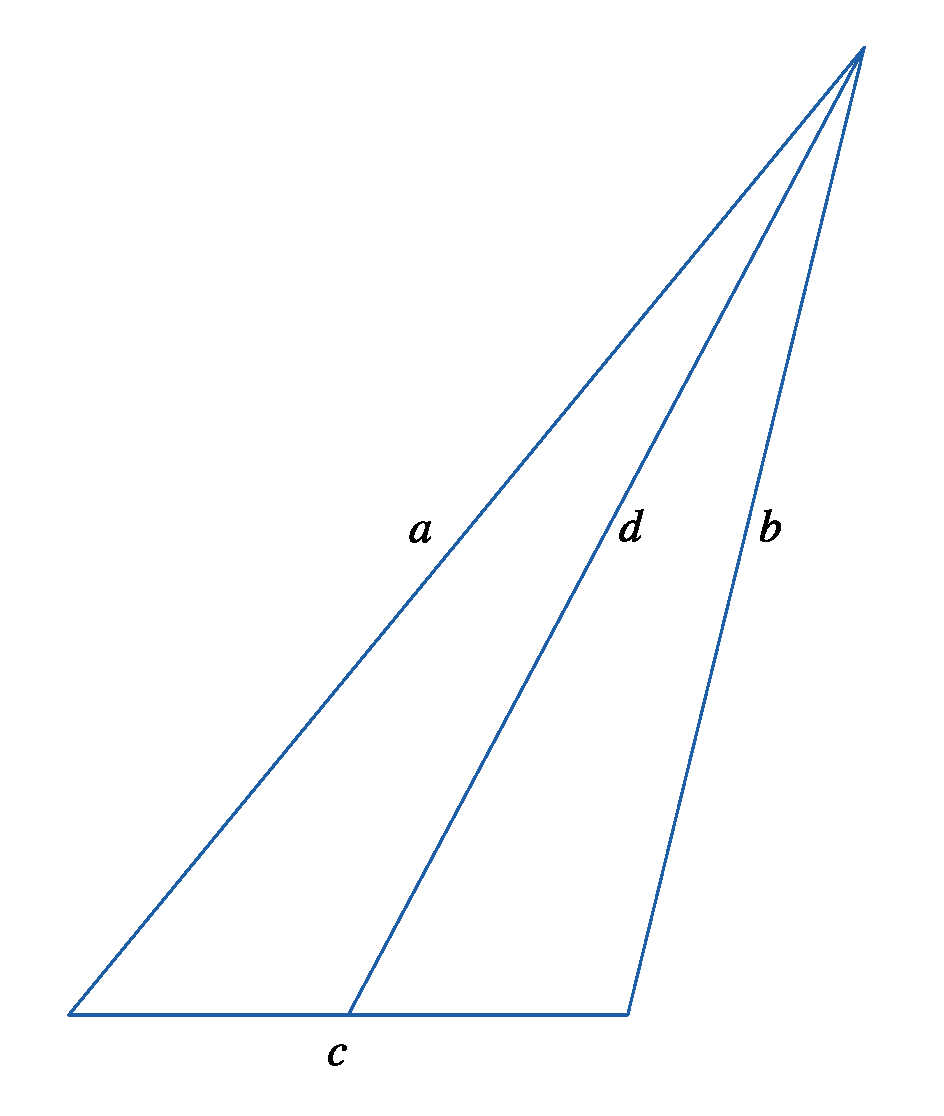
\includegraphics[width=0.3\textwidth]{median_triangle.pdf}
\end{center}

\end{exercise}

\begin{exercise}
יהיו
$a_1, \ldots, a_n,b_1, \ldots, b_n \in \RR$.
הוכיחו כי
\begin{align*}
\text{.} \prs{\sum_{k \in [n]} a_k b_k}^2 \leq \prs{\sum_{k \in [n]} k a_k^2} \prs{\sum_{k=1}^n \frac{b_k^2}{k}}
\end{align*}
\end{exercise}

\begin{exercise}
יהי
$V$
מרחב וקטורי סוף־מימדי מעל
$\RR$,
יהי
$\mcal{B} \coloneqq \prs{v_1, \ldots, v_n}$
בסיס של
$V$
ויהי
$T \in \End_\RR\prs{V}$.
הוכיחו כי לכל ערך עצמי
$\lambda \in \RR$
של
$T$
מתקיים
\begin{align*}
\text{.} \abs{\lambda}^2 \leq \sum_{\substack{j,k \in [n]}} \abs{\prs{\brs{T}_{\mcal{B}}}_{j,k}}^2
\end{align*}
\end{exercise}

\begin{exercise}
\begin{enumerate}
\item יהי
$V$
מרחב מכפלה פנימית סוף־מימדי מעל
$\RR$.
הראו כי
\begin{align*}
\trs{u,v} = \frac{\norm{u+v}^2 - \norm{u-v}^2}{4}
\end{align*}
לכל
$u,v \in V$.
זהות זאת נקראת
\emph{זהות הפולריזציה.}

\item
יהי
$V = \RR^n$
עבור
$n > 1$,
ונגדיר על
$V$
נורמה על ידי
\begin{align*}
\text{.} \norm{x}_1 = \sum_{i \in [n]} \abs{x_i}
\end{align*}

הראו כי ההעתקה
\begin{align*}
f\prs{u,v} \coloneqq \frac{\norm{u+v}_1^2 - \norm{u-v}_1^2}{4}
\end{align*}
אינה מכפלה פנימית והסיקו כי
$\norm{\cdot}_1$
אינה נורמה המושרית ממכפלה פנימית.
\end{enumerate}
\end{exercise}

\end{document}